\section{Results}
\label{sec:results}

We report task-dependent architecture behavior, delayed retention, associative retrieval and updating, component interventions, and training/execution cost under the estimands defined in Section~\ref{sec:setup}.

\subsection{Delayed Retention on Passive T-Maze}
\label{sec:tmaze_extrapolation}
How do recurrent architectures behave at the trained horizon and at longer unseen delays? We first compare established recurrent families with SdLG, then examine within-family behavior through the execution-by-phase factorial and the topology-matched formulation control.

\paragraph{Cross-family baselines.}
Table~\ref{tab:tmaze_external_main} reports terminal-policy evaluations for seven seeds of each baseline.

\begin{table*}[t]
\centering\footnotesize
\setlength{\tabcolsep}{3.5pt}
\caption{\textbf{Passive T-Maze cross-family baselines.} Mean $\pm$ sample SD over seven seeds. E/C counts early stops versus cap outcomes. Parameter counts are contextual; terminal steps do not replace horizon return.}
\label{tab:tmaze_external_main}
\begin{tabular}{lrrrrrr}
\toprule
Model & Parameters & E/C & Terminal steps (M) & $H=100$ & $H=150$ & $H=200$ \\
\midrule
GRU         & 116,227   & 1/6 & $49.012\pm2.539$ & $0.644\pm0.243$ & $0.426\pm0.345$ & $0.574\pm0.188$ \\
LSTM        & 148,995   & 0/7 & $49.971\pm0.000$ & $0.571\pm0.189$ & $0.503\pm0.008$ & $0.433\pm0.191$ \\
Mamba       & 132,611   & 0/7 & $49.971\pm0.000$ & $0.499\pm0.008$ & $0.499\pm0.008$ & $0.499\pm0.008$ \\
LTI-Linear  &  66,691   & 0/7 & $49.971\pm0.000$ & $0.501\pm0.008$ & $0.501\pm0.008$ & $0.501\pm0.008$ \\
Markovian   &  50,435   & 0/7 & $49.971\pm0.000$ & $0.506\pm0.006$ & $0.506\pm0.006$ & $0.506\pm0.006$ \\
GLA         & 1,208,195 & 7/0 & $ 5.337\pm3.852$ & $0.782\pm0.271$ & $0.782\pm0.271$ & $0.710\pm0.271$ \\
GTrXL-64    &   956,547 & 7/0 & $ 5.781\pm2.349$ & $0.930\pm0.186$ & $0.501\pm0.008$ & $0.501\pm0.008$ \\
GTrXL-128   &   956,547 & 7/0 & $ 1.428\pm0.310$ & $1.000\pm0.000$ & $0.574\pm0.188$ & $0.503\pm0.008$ \\
\bottomrule
\end{tabular}
\par\smallskip\raggedright\footnotesize
\textit{For reference,} the independently evaluated ten-seed Matched Exact condition reaches $0.900\pm0.211$, $0.900\pm0.211$, and $0.851\pm0.240$ at $H=100,150,200$, respectively (Appendix Table~\ref{tab:tmaze_overview}). These runs use a different seed set from the seven-seed baselines.
\end{table*}

GRU and LSTM show inconsistent training-horizon learning: one GRU and no LSTM runs stop early, although both $H=100$ means exceed chance. Mamba, LTI-Linear, and Markovian remain near chance. At the trained horizon $H=100$, both GTrXL configurations have higher observed means than Matched Exact: $0.930$ for GTrXL-64 and $1.000$ for GTrXL-128, versus $0.900$ for Exact. At the unseen $H=200$, the GTrXL means fall to approximately chance, whereas Matched Exact retains $0.851$; GLA has the highest baseline mean there ($0.710$).

\paragraph{Execution-by-phase factorial.}
Exact-NoRoPE reaches mean returns $0.900$, $0.900$, and $0.851$ at $H=100,150,200$; both Approximate conditions are near $0.50$ at $H=200$. The marginal Exact-minus-Approximate contrast is $0.251$ with a 95\% percentile-bootstrap interval $[0.151,0.351]$ at $H=200$ (Figure~\ref{fig:tmaze_factorial}).

\begin{figure*}[t]
\centering
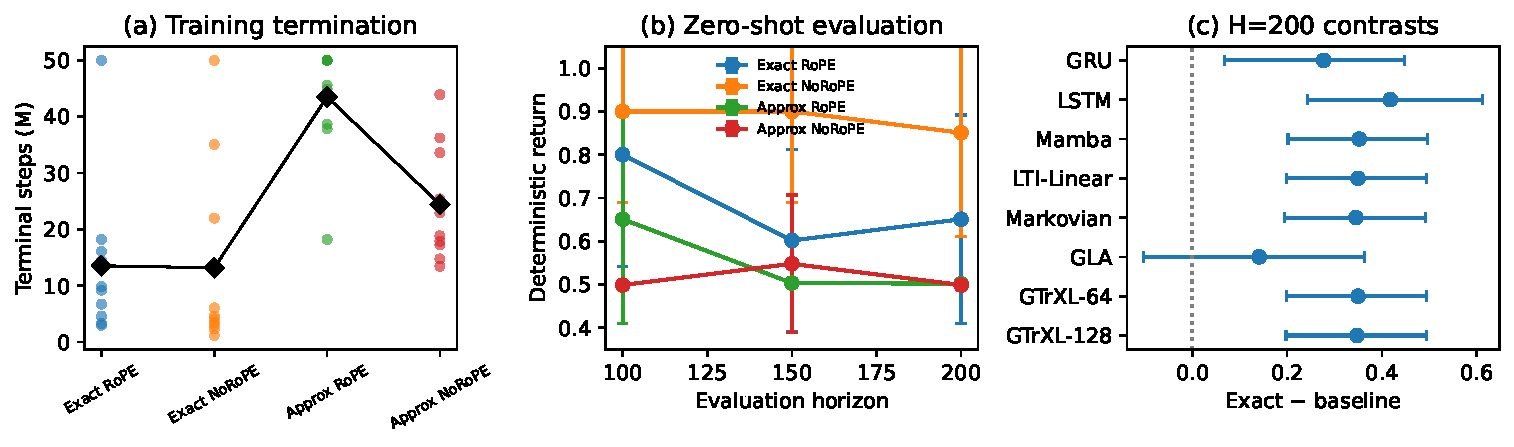
\includegraphics[width=0.74\textwidth]{plots/rebuilt/fig3_tmaze_rank_rope}
\caption{\textbf{State execution $\times$ positional phase on Passive T-Maze.} (a) Terminal steps; triangles denote capped runs, circles early stops, and bars mean $\pm$ SD. (b) Ten-seed mean return; Appendix Table~\ref{tab:tmaze_overview} gives SDs. (c) Independent-seed Exact-minus-Approximate $H=200$ contrasts; whiskers are 95\% percentile-bootstrap intervals.}
\label{fig:tmaze_factorial}
\end{figure*}

\paragraph{Matched execution.}
In the matched control, Exact reaches $0.851$ at the primary $H=200$ endpoint versus $0.500$ for Approximate, a difference of $0.351$ with a 95\% percentile-bootstrap interval $[0.200,0.497]$ (Figure~\ref{fig:tmaze_factorial}c). The comparison concerns the complete formulations rather than rank alone.

At $H=200$, the documented solve criterion classifies 7/10 Exact-NoRoPE and 0/10 Approximate-NoRoPE runs as solved in both the original factorial and matched study. Return remains primary; Appendix Table~\ref{tab:tmaze_solve_exploratory} gives post hoc exploratory Wilson intervals and Fisher tests. Early stops and terminal solves use different rollouts and thresholds and need not agree.

\subsection{Independent Associative-Memory Diagnostics}
\label{sec:results_associative}
The retrieval factorial tests a normalized Delta-rule system, while the reassignment study compares additive, fixed-gated-proxy, and normalized Delta updates on shared random associations.

\paragraph{Retrieval under associative load.}
The retrieval factorial contains ten draws in each of 48 cells over the $N,d_k,d_v$ grid defined in Section~\ref{sec:setup}.
Retrieval increases monotonically with $d_k$ in every draw at every tested load, while the $d_v$ marginal spans only $0.002$--$0.010$. It also declines systematically as $N/d_k$ grows from $0.25$ to $8$ (Figure~\ref{fig:associative_capacity}). Equal-$N/d_k$ configurations are close but not identical, with a maximum mean spread of $0.013$.

\begin{figure}[t]
\centering
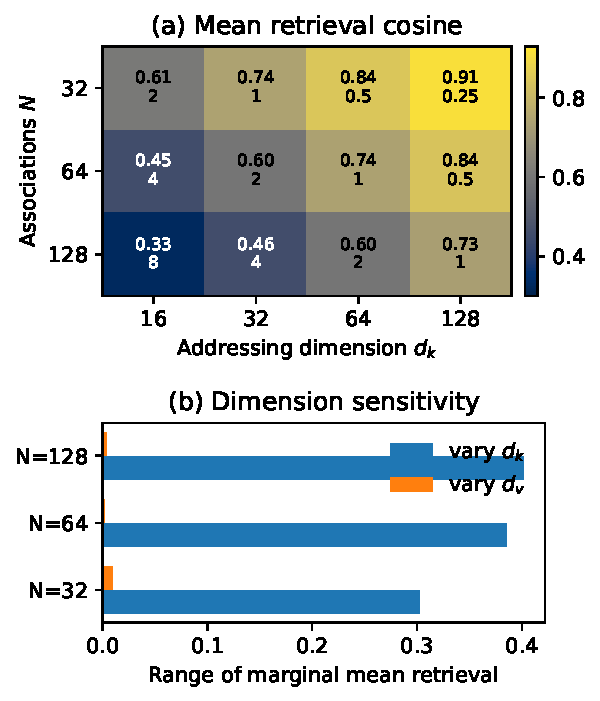
\includegraphics[width=0.78\linewidth]{plots/rebuilt/fig6_associative_capacity}
\caption{\textbf{Normalized Delta-rule retrieval diagnostic.} (a) Mean cosine by $(N,d_k)$ over $d_v$ and ten draws; sublabels give $N/d_k$. (b) Marginal ranges show greater addressing-dimension sensitivity.}
\label{fig:associative_capacity}
\end{figure}

Thus the synthetic recurrence is empirically more sensitive to addressing than value dimension under the tested random-association distribution and loads. The worst-case rank bound does not quantify this sensitivity or the capacity of learned SdLG-Exact (Appendix~\ref{app:capacity_bound_sec}).

\paragraph{Corrective reassignment.}
Does a corrective update improve replacement without damaging untouched associations? Relative to additive memory, normalized Delta updates at $\eta=0.25$ raise target fidelity from $0.502$ to $0.685$, a paired fixed-grid difference of $0.183$ with a 95\% within-cell paired-bootstrap interval $[0.181,0.185]$. Increasing $\eta$ from $0.25$ to $1.0$ adds $0.124$ in target fidelity (95\% interval $[0.122,0.127]$) but reduces non-target preservation by $0.160$ (95\% interval $[0.158,0.162]$). Stronger correction therefore improves reassignment at a measurable cost to untouched associations under this protocol. The fixed-gated proxy and complete method table appear in Appendix~\ref{app:component_transfer}.

\subsection{Task-Dependent Architecture Ordering}
\label{sec:popgym_results}
\paragraph{DoorKey-8x8 comparison.}
Across five seeds per model, Exact has the highest mean terminal return and success rate and the most early stops (three versus two for GTrXL and one for GRU; Table~\ref{tab:doorkey_8x8_main}).

\begin{table}[t]
\centering\footnotesize
\setlength{\tabcolsep}{3pt}
\caption{\textbf{DoorKey-8x8 terminal-policy evaluation.} Five-seed mean $\pm$ sample SD; E/C counts early stops versus caps. Appendix~\ref{app:doorkey_8x8} gives individual runs.}
\label{tab:doorkey_8x8_main}
\begin{tabular}{lrrr}
\toprule
Model & Eval. return & Success rate & E/C \\
\midrule
SdLG-Exact & $0.668\pm0.408$ & $0.748\pm0.362$ & 3/2 \\
PPO-GRU & $0.193\pm0.432$ & $0.200\pm0.447$ & 1/4 \\
PPO-GTrXL & $0.468\pm0.466$ & $0.537\pm0.446$ & 2/3 \\
\bottomrule
\end{tabular}

\end{table}

\paragraph{POPGym task comparisons.}
The POPGym evaluations~\cite{morad2023popgym} use each seed's maximum logged evaluation return, with three seeds for the multi-seed task comparisons discussed here. Exact exceeds GRU on CountRecall (accumulation/query) but is lower on Concentration (discrete matching), MinesweeperEasy ($0.591$ versus $0.942$), and LabyrinthEscapeEasy ($0.671$ versus $0.971$; Appendix Table~\ref{table:popgym_easy_full}). The two SdLG formulations also change order by task: Exact exceeds Approximate on CountRecallEasy ($0.670$ versus $-0.712$), whereas Approximate is higher on ConcentrationEasy ($-0.102$ versus $-0.267$) and LabyrinthEscapeEasy ($0.967$ versus $0.671$; Appendix Table~\ref{table:popgym_easy_full}).

\subsection{Component Interventions}
\label{sec:optional_controls}

\paragraph{Local pathway in SdLG-Approximate.}
On XLand-MiniGrid MemoryS16, SWA enabled has mean return $0.508$ (SD $0.445$), versus $0.782$ (SD $0.354$) when bypassed; the enabled-minus-bypassed difference is $-0.274$ with a 95\% independent-bootstrap interval $[-0.549,0.008]$ over 15 runs per condition (Appendix Figure~\ref{fig:minigrid_ablation}). The interval includes zero.

\paragraph{Actor-gradient scaling in the Hybrid configuration.}
At 20.15M steps, $\alpha=0.1$ has mean return $11.210$ versus $9.757$ for $\alpha=1.0$. All five matched pairs favor attenuation (Figure~\ref{fig:ggs_telemetry}); the paired difference is $1.453$ with a 95\% percentile-bootstrap interval $[0.925,1.962]$. This interval is conditional on the five observed pairs; with five pairs, the smallest attainable two-sided exact sign-flip $p$-value is $0.0625$. Probe cosine remains descriptive rather than a PPO-loss-conflict measure.

\begin{figure}[t]
\centering
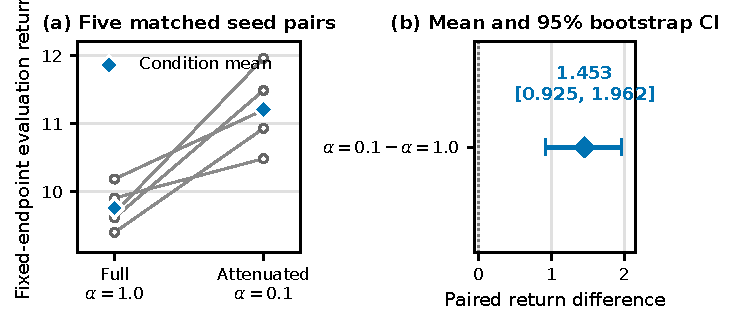
\includegraphics[width=0.70\linewidth]{plots/gradient_shielding_paired.pdf}
\caption{\textbf{Actor-gradient scale on Craftax.} (a) Five matched-seed endpoint returns; lines join common initializations and random streams, and diamonds mark means. (b) Attenuated-minus-full paired mean and exact percentile-bootstrap 95\% interval.}
\label{fig:ggs_telemetry}
\end{figure}

\subsection{Training-Configuration and Systems Behavior}
\label{sec:systems_results}

\paragraph{Rollout/TBPTT-length response.}
Do architecture orderings depend on the rollout/TBPTT configuration?
The Craftax cross-$T$ results report five-run final logged training-return means after a 50M-step budget (Figure~\ref{fig:craftax_cross_t}). SdLG-Approx changes from $16.33\pm0.37$ at $T=16$ to $14.79\pm0.36$ at $T=64$, while PPO-GLA reaches $15.69\pm0.22$ at $T=64$. Ordering varies with $T$, which jointly changes rollout, TBPTT, GAE, and update structure.

\begin{figure}[t]
\centering
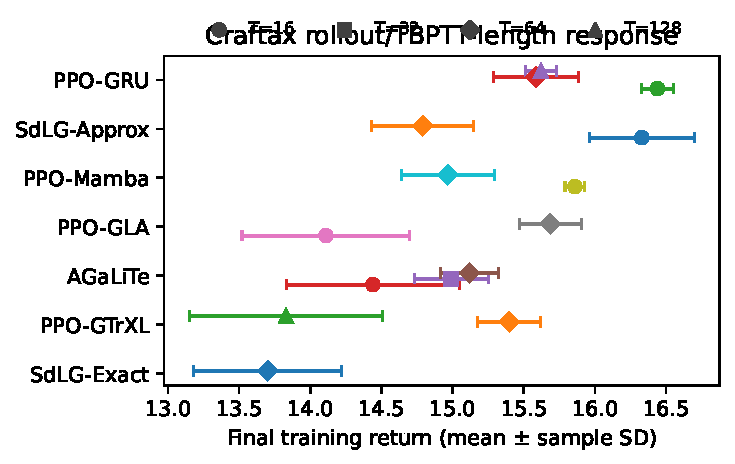
\includegraphics[width=0.72\linewidth]{plots/rebuilt/fig7_craftax_cross_t.pdf}
\caption{\textbf{Craftax rollout/TBPTT-length response.} Five-run final logged training-return mean $\pm$ SD after a 50M-step budget. Markers identify rollout/TBPTT length $T$; blank cells were not run. SdLG-Approx is logged as \texttt{SdLGHybrid} with a coupled trunk.}
\label{fig:craftax_cross_t}
\end{figure}

\paragraph{Fixed-$T$ return and training-loop throughput.}
At $T=64$ and 50M steps, PPO-GRU ($0.81$M parameters) reaches return $15.59$ and 25.2k loop steps/s; the other four models span $14.97$--$15.69$ and 10.0k--17.8k steps/s. Exact reaches $13.70\pm0.52$ across five runs; its measured cumulative training-loop throughput is approximately 9.4k environment steps/s. These are cumulative loop measurements, not recurrent-step latency or kernel throughput.

\paragraph{Matched recurrent-state and inference cost.}
Under a matched three-block topology, Approximate carries 24,780 bytes per environment versus 62,988 for Exact, a $60.7\%$ reduction. Median warmed latency is $0.984$ versus $0.960$ ms at batch 256 and $0.675$ versus $0.586$ ms at batch 1 (300 iterations after 50 warm-ups on ROCm). Factorization saves state without reducing latency; bytes exclude parameters, activations, and allocation overhead (Appendix~\ref{app:component_transfer}).
